\section{Phân tích sai số theo lớp}
Ma trận nhầm lẫn được tạo từ toàn bộ 10.000 dự đoán ngoài mẫu, không lấy từ tập huấn luyện. Tập test có 7.319 mẫu High, 2.587 mẫu Moderate và 94 mẫu Low. MLP dự đoán đúng 6.733 mẫu High, 1.440 mẫu Moderate nhưng chỉ 7 mẫu Low. Vì vậy accuracy 81,8\% che giấu khả năng nhận diện lớp hiếm còn yếu. Recall của Low chỉ khoảng 7,45\%; kết quả này cho thấy hạn chế đáng kể ở lớp hiếm.
\begin{figure}[htbp]\centering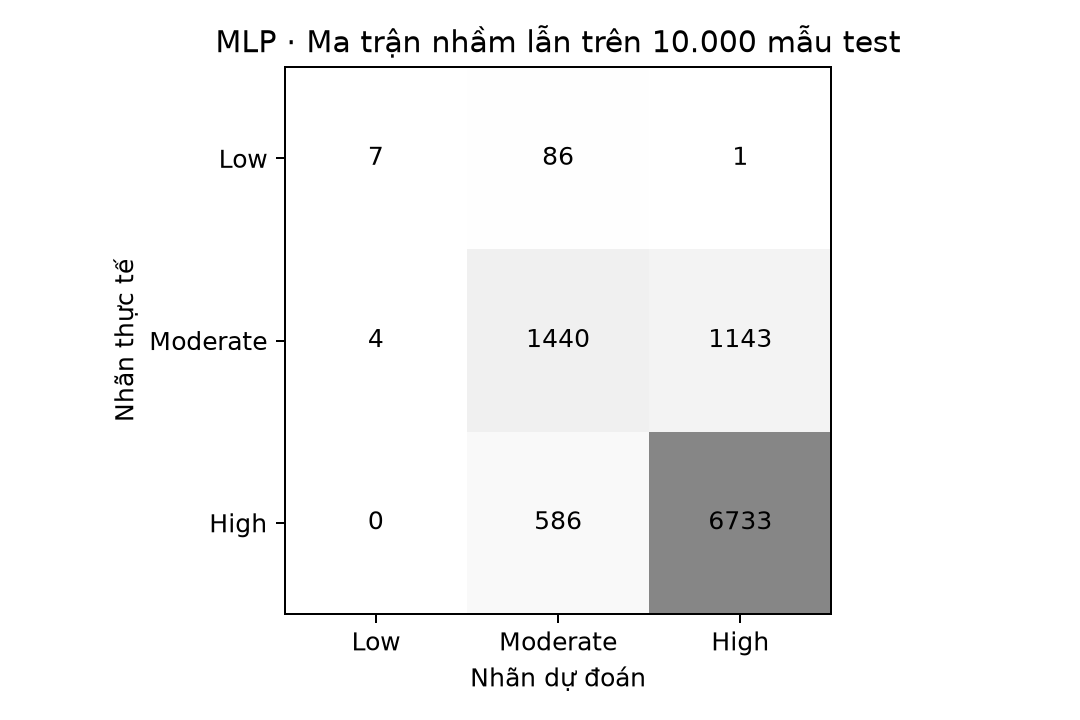
\includegraphics[width=.85\linewidth]{figures/confusion.png}\caption{Ma trận nhầm lẫn của MLP trên tập kiểm tra phân tầng.}\end{figure}
Tỷ lệ lỗi giữa Moderate và High cho thấy ranh giới của nhãn tổng hợp chưa được mô hình tách tốt. Cải thiện tiếp theo cần so sánh trọng số lớp, điều chỉnh ngưỡng và cách lấy mẫu trên validation, đồng thời giữ nguyên test để tránh chọn cấu hình theo kết quả test. Không đổi tên nhãn tổng hợp thành chẩn đoán y tế.
\section{Phân tích phần dư hồi quy}
\begin{figure}[htbp]\centering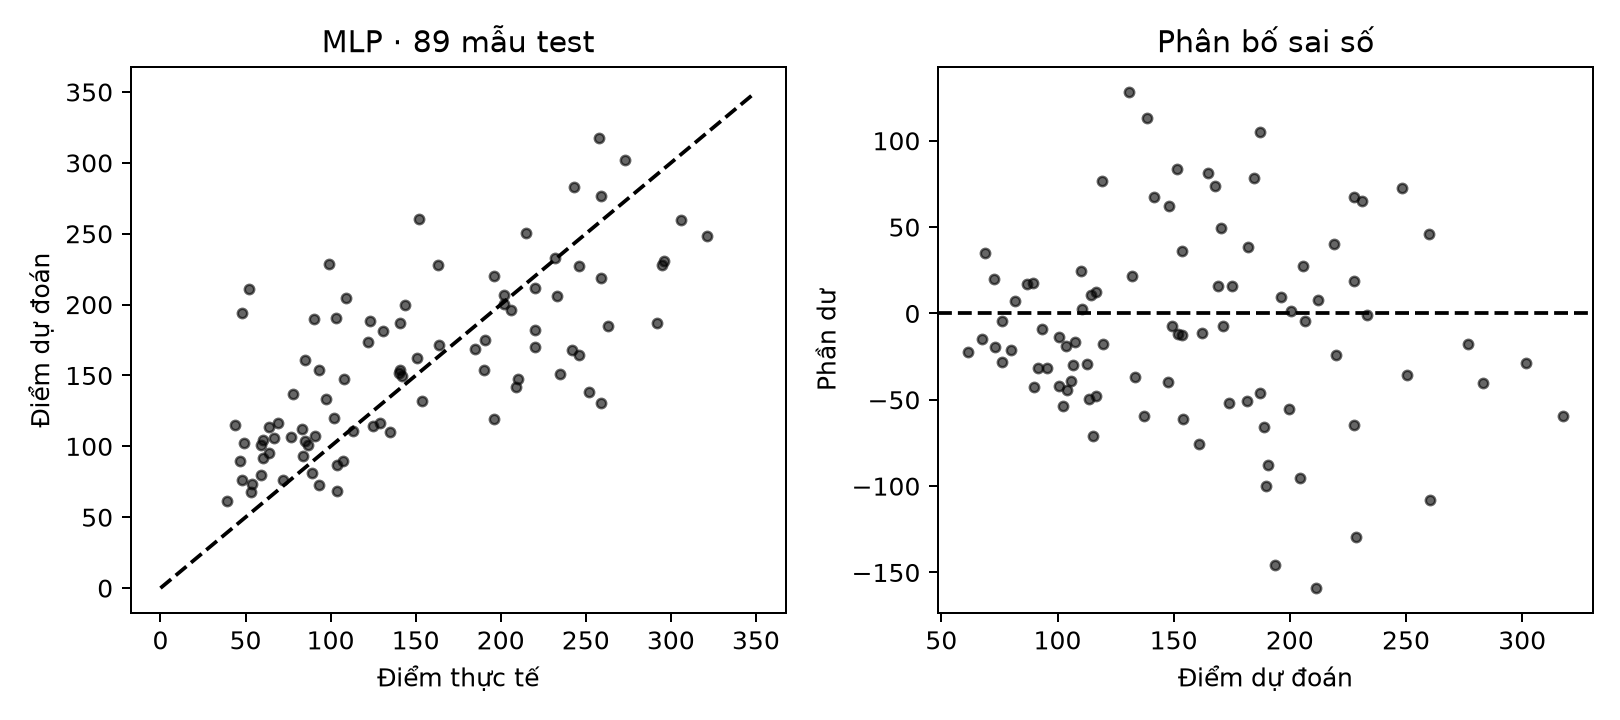
\includegraphics[width=\linewidth]{figures/regression.png}\caption{Dự đoán và phần dư của MLP trên 89 mẫu kiểm tra.}\end{figure}
Đường chéo thể hiện dự đoán bằng giá trị thật. Những điểm cách xa đường chéo đóng góp lớn vào MAE. Phần dư được tính bằng giá trị thực trừ dự đoán; phần dư dương biểu thị dự đoán thấp hơn thực tế. Không thể dùng một chỉ số tổng hợp để bảo đảm mọi nhóm đầu vào có sai số tương đương. Bản này chưa xây dựng khoảng dự báo và chưa hiệu chỉnh bất định.
\section{Hợp đồng dữ liệu và API}
GET /api/schema cung cấp thứ tự đặc trưng. GET /api/examples cung cấp một mẫu từ mỗi bộ dữ liệu để trình diễn. POST /api/chat nhận question, task và values. Với task knowledge, hệ thống truy xuất văn bản; với classification hoặc regression, values phải đủ các trường tương ứng. Kết quả gồm answer, result, sources, graph\_evidence và trace.

Trường result của phân loại gồm label, scores và scope. scores là đầu ra xác suất lớp của mô hình trên nhãn tổng hợp, chưa được hiệu chỉnh. Trường result của hồi quy gồm value và scope. Việc tách cấu trúc này tránh dùng chung một con số cho hai ý nghĩa khác nhau. Dữ liệu mẫu là mẫu của bộ nghiên cứu, không phải hồ sơ do người dùng cung cấp.

Nút ``Giải thích kết quả'' trên web gửi lại task và values của mẫu vừa chạy, nên câu trả lời được tính từ chính các đầu vào đó. Nhánh phân loại nêu nhãn, điểm của ba lớp, accuracy và macro-F1 trên tập test; nhánh hồi quy nêu điểm tiến triển, MAE và $R^2$. Mỗi nhánh đều giải thích ý nghĩa của nhãn/điểm và giới hạn khi chuyển sang trường hợp cá nhân. Mã tạo diễn giải nằm trong \path{app/model_explanation.py}; nó không sinh khuyến nghị điều trị.

Kiểm tra đầu vào hiện yêu cầu số hữu hạn, giới hạn trị tuyệt đối và đủ số trường. Đây là kiểm tra kỹ thuật, chưa phải kiểm định lâm sàng từng đơn vị. Giá trị nhập bằng số nhưng sai đơn vị vẫn có thể làm kết quả vô nghĩa; vì vậy demo được giới hạn ở dữ liệu nghiên cứu và có nút điền mẫu.
\section{Kết quả kiểm thử tích hợp}
Script test\_scenarios.py thực hiện tám trường hợp: câu hỏi có nguồn; câu hỏi ngoài từ vựng; suy luận phân loại; suy luận hồi quy; thiếu trường; giá trị không hữu hạn; tên bài toán không hợp lệ; lỗi Neo4j có kiểm soát. Tám trường hợp đều đạt điều kiện kiểm tra ở lần chạy lưu trong results/api\_scenarios.json. Kiểm tra lỗi cơ sở dữ liệu được thực hiện bằng thay thế driver trong test, không phải chủ động tắt cơ sở dữ liệu đang phục vụ người dùng.

Kiểm thử xác nhận hợp đồng phản hồi và nhánh lỗi, chưa đo độ chính xác truy xuất trên tập câu hỏi lớn. Trường hợp ngoài miền sử dụng chuỗi không có trong từ vựng, do đó không chứng minh hệ thống phát hiện mọi câu hỏi ngoài miền bằng tiếng Việt. Những giới hạn này giúp tách kiểm thử chức năng khỏi đánh giá chất lượng tư vấn.

Bản cập nhật thêm bảy điều kiện trong \path{scripts/test_chat_upgrade.py}: bốn chủ đề RAG mới, hai cách diễn giải kết quả mô hình và tổng số tài liệu công bố qua API. Thử nghiệm xác nhận các đoạn dẫn đúng nguồn và không biến điểm nghiên cứu thành chẩn đoán. Đây vẫn là kiểm tra chức năng theo kịch bản, chưa phải đánh giá y khoa bởi chuyên gia.
\section{Đối chiếu với sơ đồ yêu cầu}
\begin{longtable}{p{4cm}p{10cm}}\toprule Thành phần & Hiện thực trong sản phẩm\\\midrule
DB và Deep Learning & Hai bộ dữ liệu tách biệt, MLPClassifier và MLPRegressor; có checkpoint và kết quả test.\\
Phân loại và dự đoán & Hai lựa chọn trong phòng thực nghiệm, cùng chuyển kết quả đến phản hồi và nhật ký.\\
Web/sách đến KB & Kế thừa KB đã biên soạn từ tiểu luận 02; bảo toàn mã nguồn tài liệu, không tự động thu thập web ở thời điểm chạy.\\
KB và RAG & TF-IDF chọn đoạn văn; Neo4j trả các quan hệ cùng mã tài liệu; phản hồi trích đoạn có nguồn.\\
Agent và RL + rule & Handler và MessageBus xử lý yêu cầu; chính sách học một bước chọn kiểu phản hồi, luật chặn thiếu bằng chứng.\\
Tư vấn, trợ giúp & Chatbot giải thích kiến thức và phạm vi đầu ra; bản local dùng Qwen LoRA cho câu kiến thức có nguồn, còn câu thông số và thuốc theo luật.\\\bottomrule\end{longtable}
